\documentclass[a4paper,kulak]{kulakarticle}

\usepackage[utf8]{inputenc}
\usepackage[dutch]{babel}

\usepackage{float}
\usepackage{subfig}

\date{Academiejaar 2017-2018}
\address{
  Naam van de opleiding \\
  Naam van het vak \\
  Naam van de docent/begeleiders}
\title{Titel van het document}
\author{Naam van de auteurs}

\begin{document}

\maketitle

\section*{Motivatie}



\section{Onze oplossing}

\subsection{Achtergrondverwijdering}
Het eerste deel van ons project is de achtergrond van de bloedklonters te verwijderen. Op de afbeeldingen is er heel wat vuiligheid te vinden. Een voorbeeld hiervan zijn luchtbellen of kleine bloedklonters zoals men ziet op de volgende figuur \ref{figuur achtergrondverwijdering}. Hieronder zullen we verschillende operaties beschrijven om de grootste klonters te lokaliseren en alles dat geen klonter is te verwijderen. Dit leidt tot een ruisvrije afbeelding.

\begin{figure}[H]
	\centering
	\includegraphics[width = \textwidth]{Ruis_afbeelding.png}
	
	\caption{In de rechterbovencirkel zien we luchtbellen en in de onderste cirkel zien we een verkleuring die geen deel uitmaakt van een bloedklonter.}
	\label{figuur achtergrondverwijdering}
\end{figure}

\subsubsection{Bepalen van de beste treshold}
Wanneer we de grijswaarden van de afbeelding berekenen, zien we een duidelijk verschil tussen de achtergrond (eerder wit) en de bloedklonter (eerder grijs) zoals we zien op figuur \ref{figuur beste_treshold}. Wanneer we een histogram van deze grijswaarden opstellen, vinden we ook dat er een lokaal minimum is tussen het grijs en het wit. Dit zien we duidelijk op het histogram \ref{figuur graf1}. Wanneer we dit minimum berekenen vinden we de theoretisch optimale treshold, de waarde om een bloedklonterpixel van een achtergrondpixel te onderscheiden. Wanneer we die treshold toepassen en een binaire representatie zoals figuur \ref{figuur foto_bin} vormen, zien we duidelijk dat dit een goede treshold is.

\begin{figure}[H]
	\centering
	\subfloat[]{{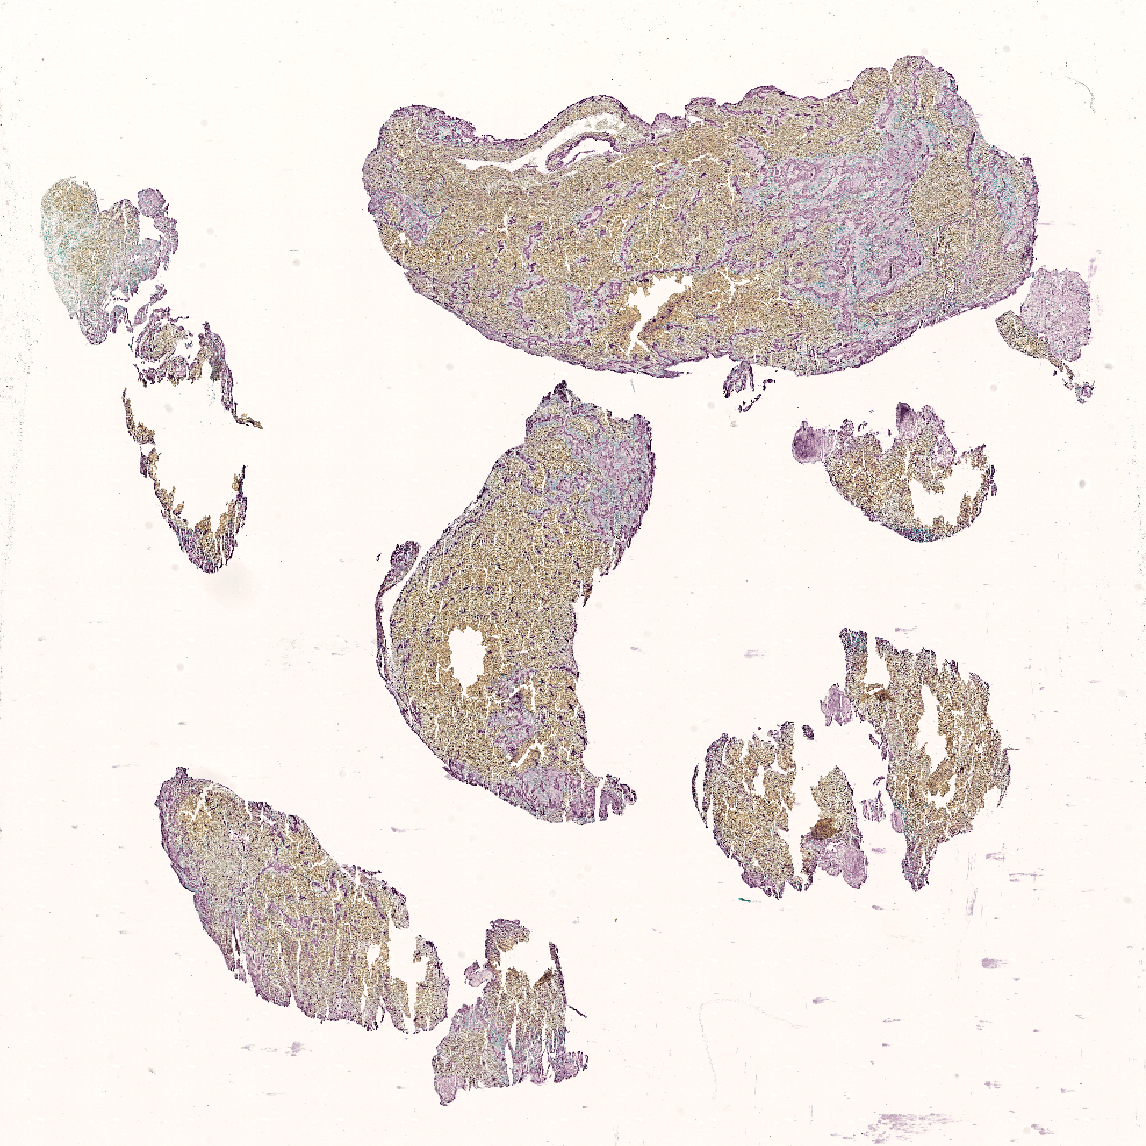
\includegraphics[height=8cm]{origineel_vb}}}
	\subfloat[]{{\includegraphics[height=8cm]{grijswaarden_vb}}}
	
	\caption{Illustratie van de originele foto (a) en deze omgezet in grijswaarden (b)}
	\label{figuur beste_treshold}
\end{figure}

\begin{figure}[H]
	\centering
	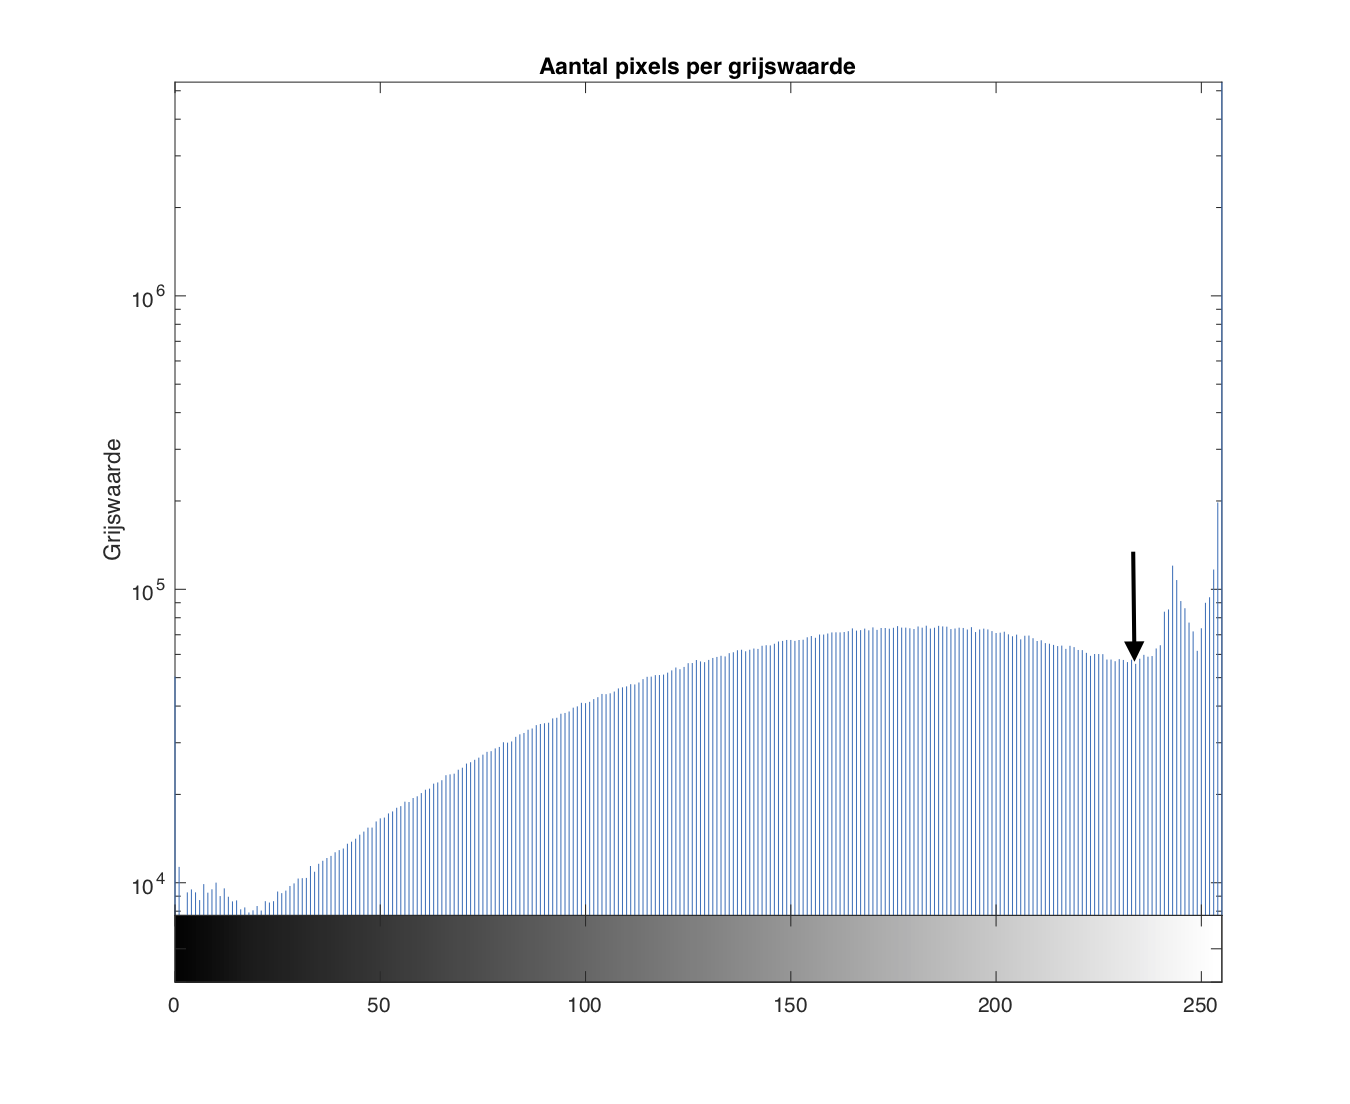
\includegraphics[width=0.85\textwidth]{GetBestTreshold_vb_aangeduid.png}
	
	\caption{Histogram van het aantal pixels gegroepeerd per grijswaarde. We zien duidelijk een lokaal minimum rond de waarde 230. Opmerking: we maken hier gebruik van een logaritmische y-as.}
	\label{figuur graf1}
\end{figure}
\begin{figure}[H]
	\centering
	\includegraphics[width=0.7\textwidth]{grijswaarden_bin_vb}
	
	\caption{Op deze binaire representatie zijn de bloedklonters duidelijk te zien}
	\label{figuur foto_bin}
\end{figure}

\subsubsection{Lokaliseren van de bloedklonters}
Eenmaal deze binaire representatie gevonden is, lokaliseren we de grootste klonters om het ruis te verwijderen. Hiervoor zullen we eerst alle holtes in de klonters opvullen door alle ingesloten pixels\footnote{Een ingesloten pixel is een zwarte pixel die onmogelijk de achtergrond van de afbeelding kunnen bereiken zonder over witte pixels te gaan} wit te maken. Het resultaat is te zien in figuur \ref{figuur lok_bloed}. De klonters zijn nu nog veel duidelijker zichtbaar, waardoor we kunnen overgaan naar de effectieve ruisfilter.

\begin{figure}[H]
	\centering
	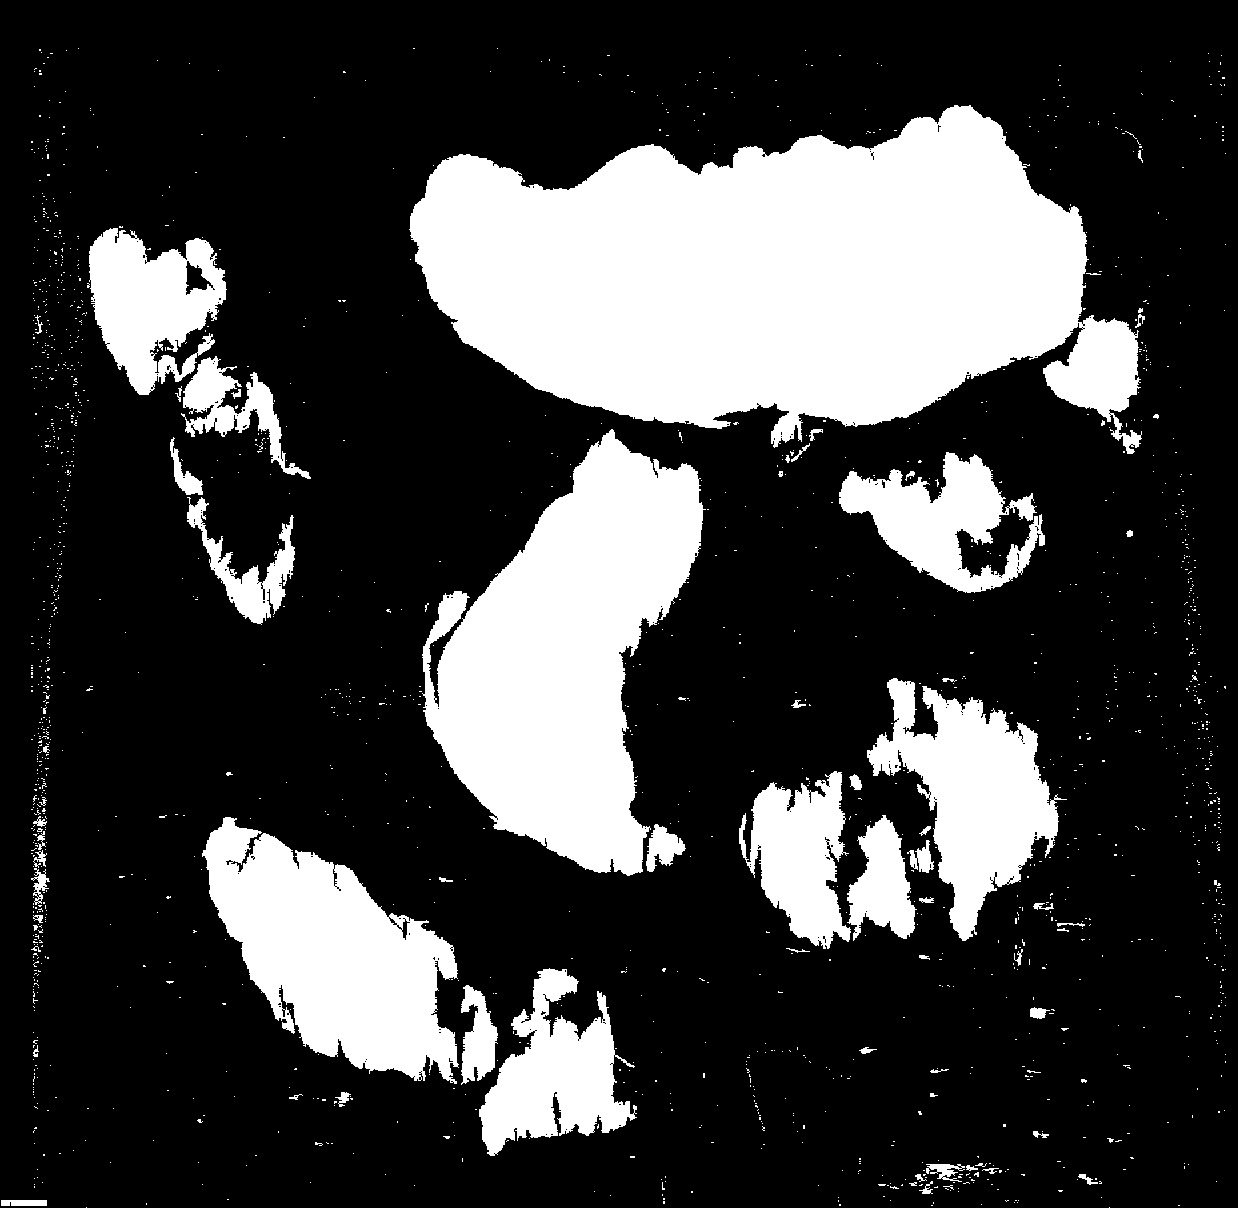
\includegraphics[width = 0.7\textwidth]{grijswaarden_bin_gevuld_vb}
	
	\caption{Alle gaatjes zijn nu opgevuld, waardoor we de grootte van de bloedklonters kunnen berekenen}
	\label{figuur lok_bloed}
\end{figure}

\subsubsection{Ruisfilter}
Voor de ruisfilter verwijderen we elke groep witte pixels met een omvang kleiner dan een constante waarde. Indien dit zo is, worden de witte pixels door zwarte vervangen. Dit simpel algoritme verwijdert alle ruis zoals te zien is in figuur \ref{figuur ruisfilter}. Deze zogenaamde 'mask' kunnen we toepassen op de originele afbeelding om officieel het ruis te verwijderen.

\begin{figure}[H]
	\centering
	\subfloat[]{{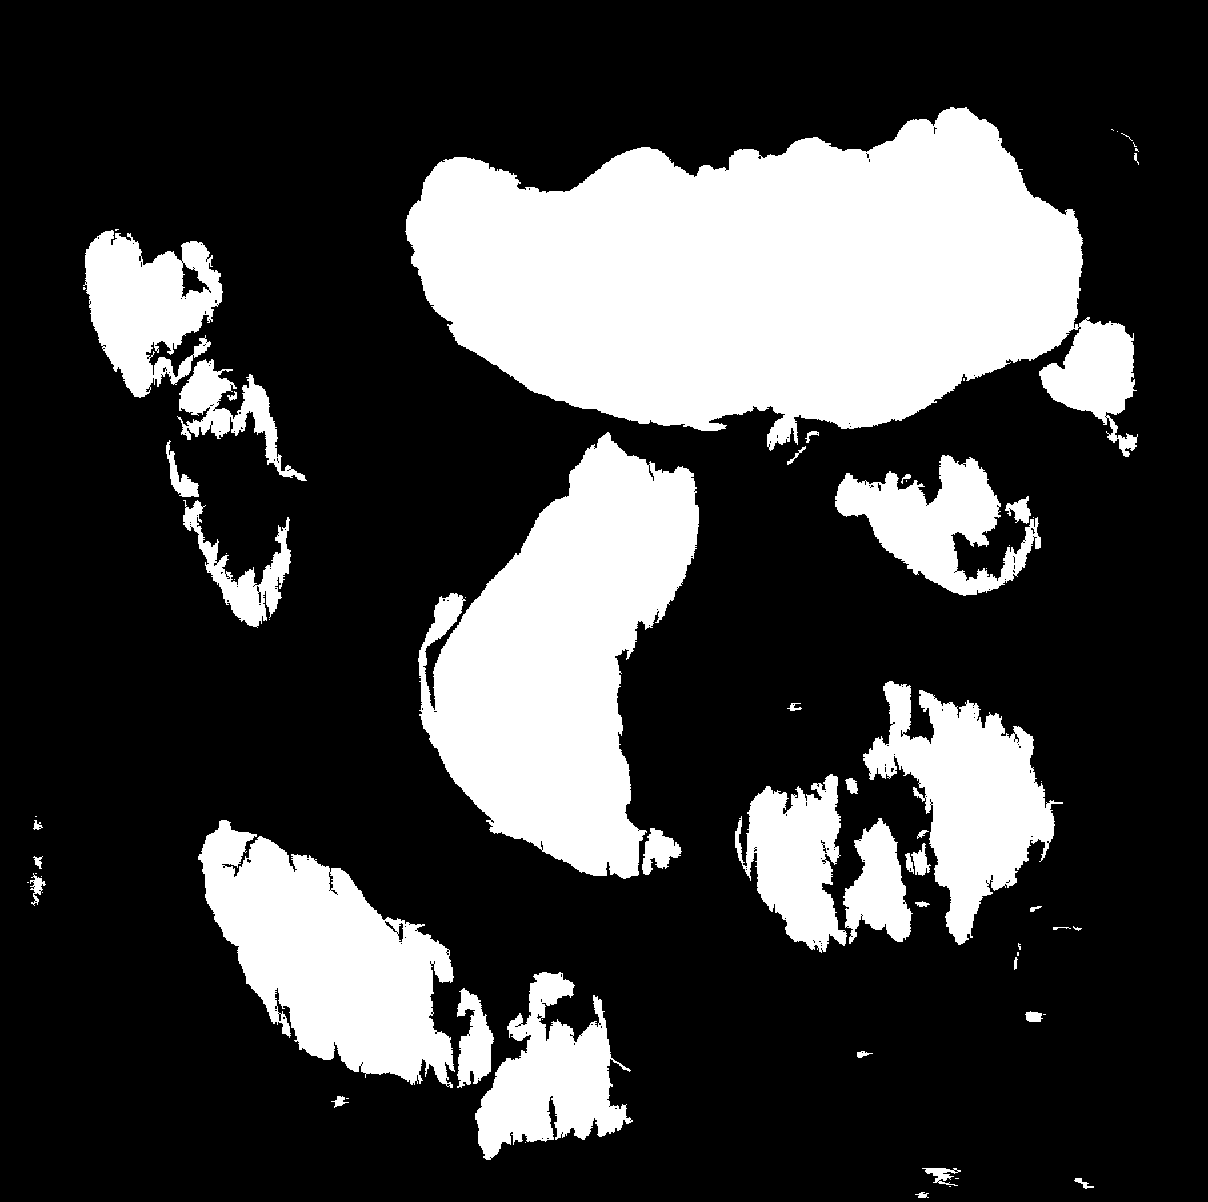
\includegraphics[width=8cm]{ruisvrij_vb}}}
	\subfloat[]{{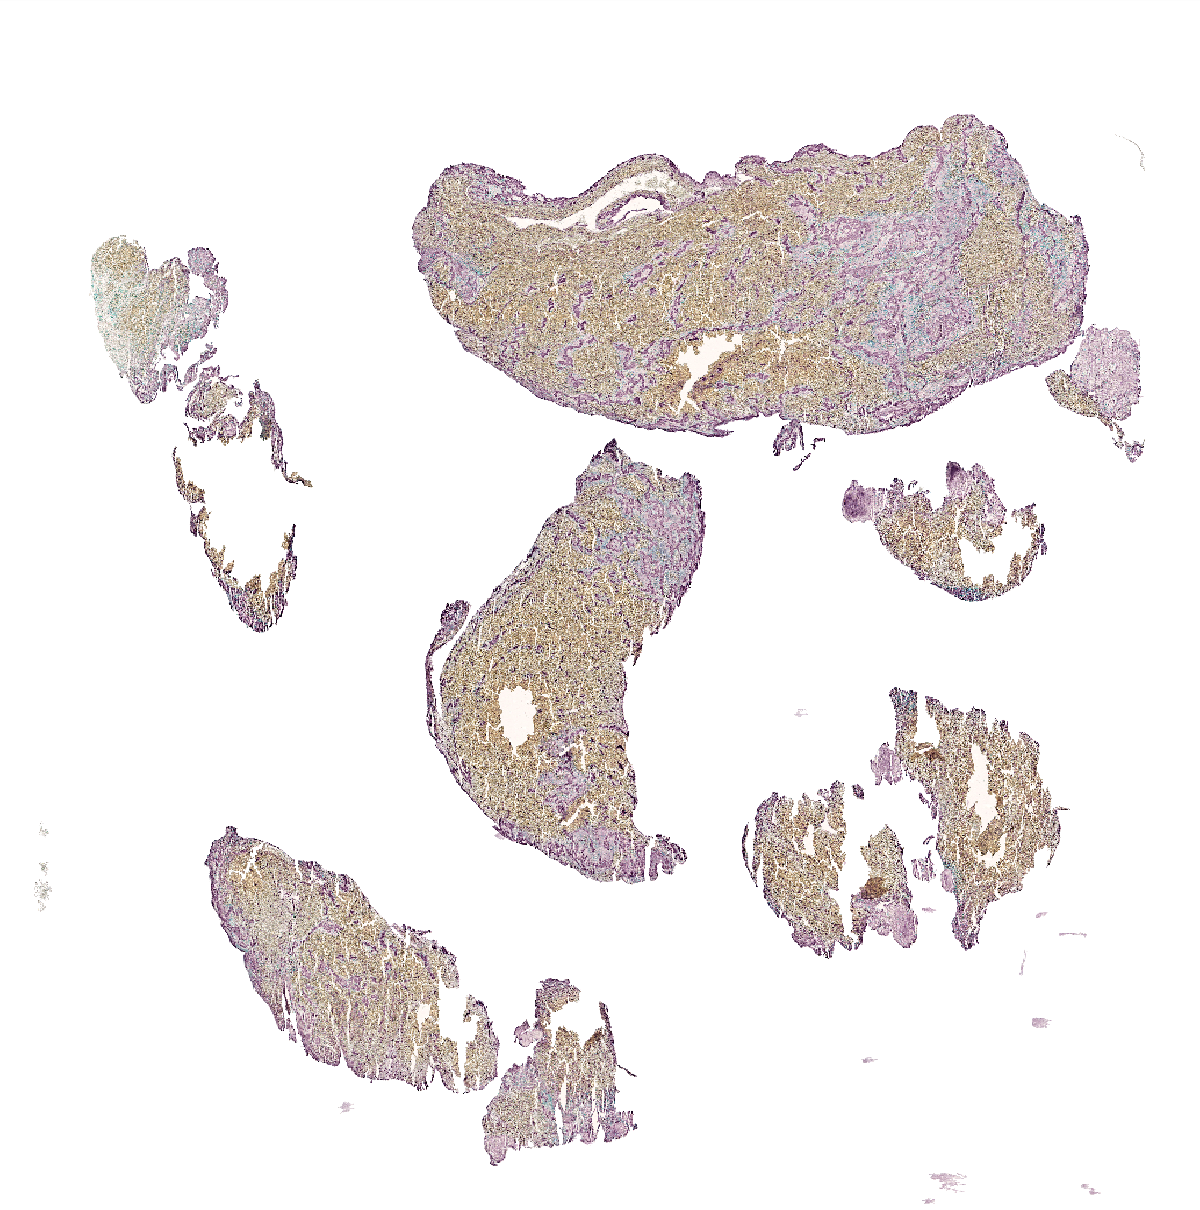
\includegraphics[width=8cm]{ruisvrij_kleur_vb}}}
	
	\caption{Alle ruis is verwijderd, dit is een foto waarmee we kunnen werken}
	\label{figuur ruisfilter}
\end{figure}

\subsection{Lokalisatie van de indicator}
Het tweede deel van ons project is de indicators lokaliseren. We hebben de opdracht gekregen twee soorten te kunnen onderscheiden. Een voorbeeld van deze twee is op de volgende figuren \ref{figuur indicators} te zien. Omdat het kleurverschil tussen indicator en achtergrond niet altijd even groot is, vormen we het oorspronkelijke \textit{RGB} kleurmodel \footnote{Het RGB kleurmodel is een voorstelling waarbij ieder kleur voorgesteld wordt door een waarde van de drie basiskleuren(rood, groen en blauw)} om naar het zogenaamde \textit{HSV} kleurmodel. Dit model is een alternatieve voorstelling waarbij men alle kleuren op een cirkel voorstelt, de hoek die dit kleur maakt, noemt men de \textit{Hue}. Naast deze waarde heeft \textit{HSV} nog twee andere parameters namelijk \textit{Saturation} en \textit{Value}. \textit{Saturation} kan simpel beschouwd worden als een aanduiding van de hoeveelheid witte kleur en \textit{Value} een aanduiding van de zwarte kleur. Een grafisch overzicht is te zien op figuur \ref{figuur hsv_schema}.\\
Het voordeel van deze transformatie is dat het heel wat eenvoudiger is om een onderscheid tussen dichtbijgelegen kleuren te vinden. Een andere mogelijke transformatie is die naar het \textit{Lab} kleurmodel die gelijkaardige eigenschappen heeft en desnoods ook gebruikt kan worden. Eenmaal we een duidelijk onderscheid tussen de indicator en de achtergrond maken, kunnen we eenvoudig het percentage indicator berekenen door het aantal bloedklonter- en indicatorpixels op te tellen. Ons stappenplan wordt in volgende hoofdstukken besproken en wordt toegepast op de afbeelding uit figuur \ref{figuur indicators} (a).
\begin{figure}[H]
	\centering
	\subfloat[]{{\includegraphics[width=7.5cm]{Indicator_vb1}}}
	\qquad
	\subfloat[]{{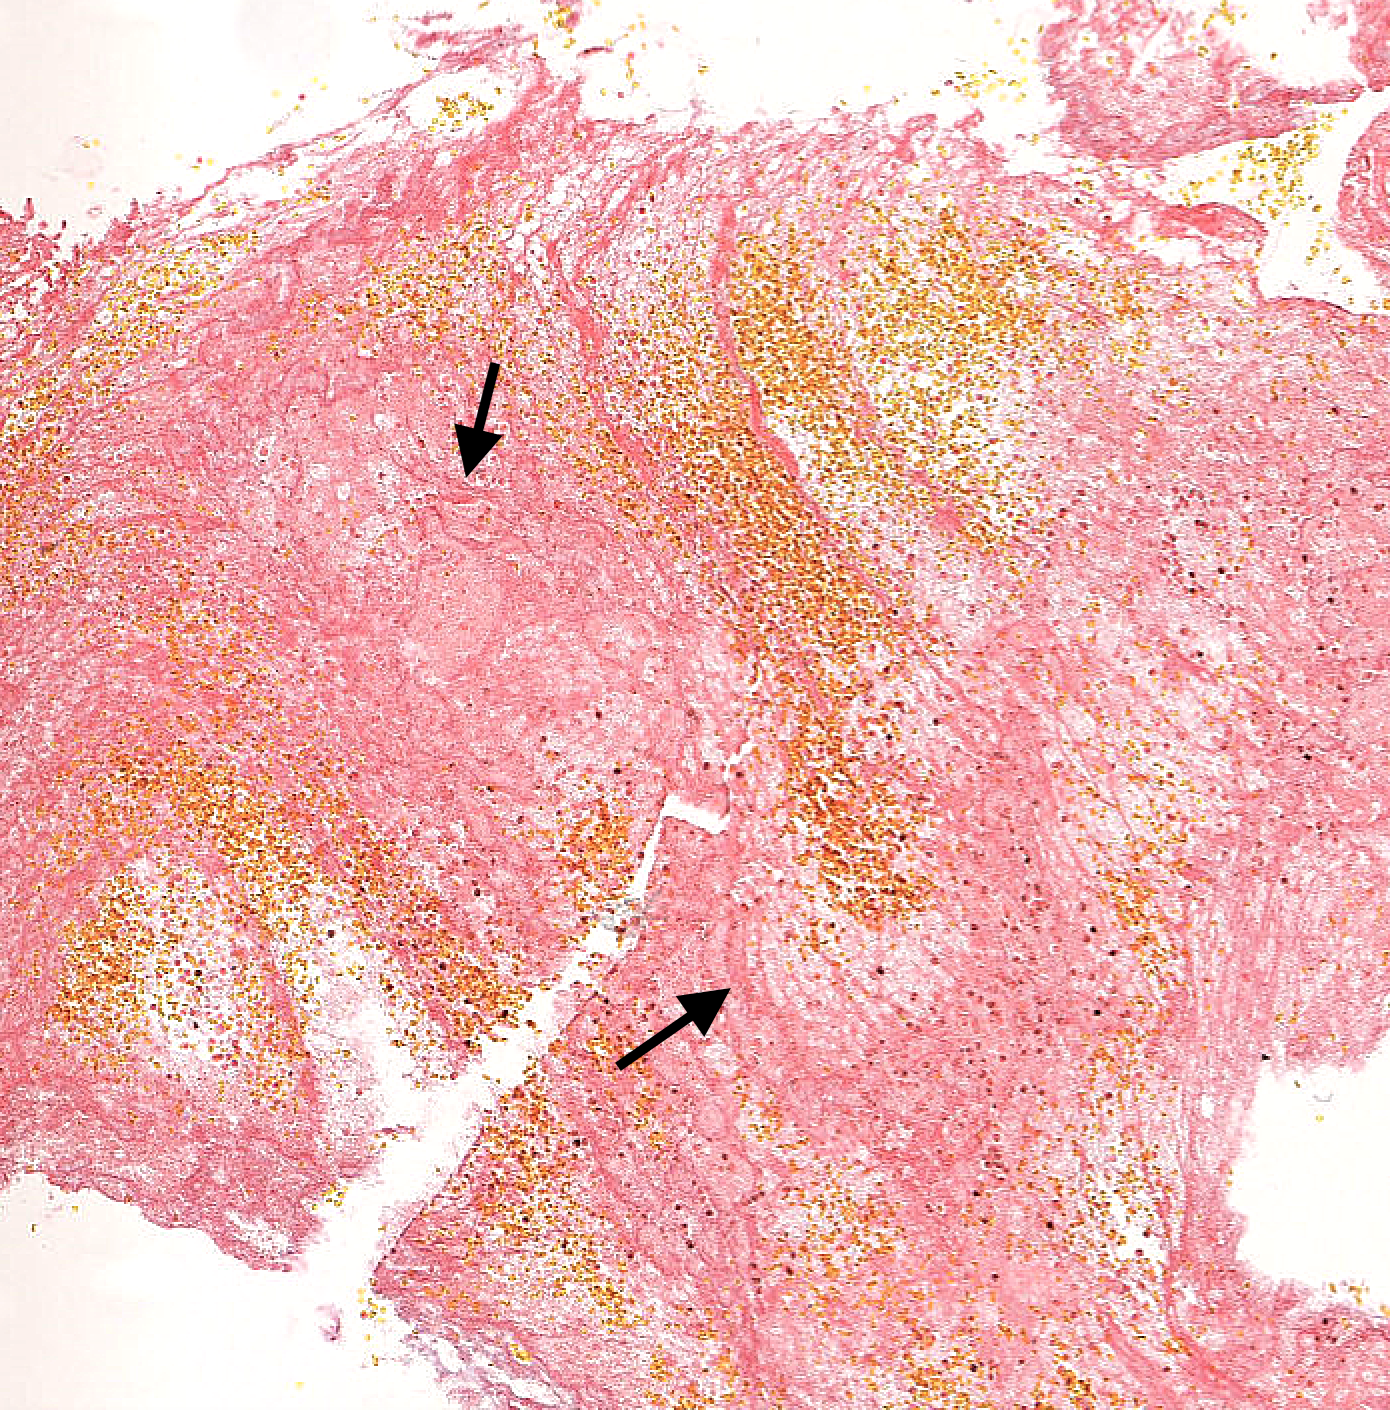
\includegraphics[width=7.5cm]{Indicator_vb2}}}
	
	\caption{Illustratie van de twee soorten indicator (respectievelijk paars en donkerroze) die gedetecteerd moeten worden. We zien duidelijk dat het detecteren op afbeelding (a) eenvoudiger zal zijn dan op afbeelding (b)}
	\label{figuur indicators}
\end{figure}
\begin{figure}[H]
	\centering
	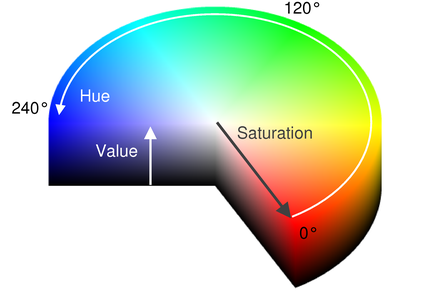
\includegraphics[width=0.7\textwidth]{HSV_vb.png}
	
	\caption{Grafische voorstelling van het HSV (Hue, Saturation, Value) kleurmodel}
	\label{figuur hsv_schema}
\end{figure}

\subsubsection{het HSV kleurmodel}
Zoals reeds vermeld, beginnen we met een transformatie naar het \textit{HSV} kleurmodel. Bijgevolg kunnen we de twee voorstellingen vergelijken. We hebben het model telkens ontbonden in de drie kleurwaarden, waarbij zwart de laagste waarde voor dat kleur is en wit de hoogste. De resultaten zijn te zien in de figuren \ref{figuur RGB} en \ref{figuur HSV}. Het verschil tussen de twee kleurmodellen is duidelijk te zien, afbeelding (a) en (b) uit figuur \ref{figuur HSV} lijken namelijk iets agressiever een onderscheid tussen de kleuren te maken.

\begin{figure}[H]
	\centering
	\subfloat[]{{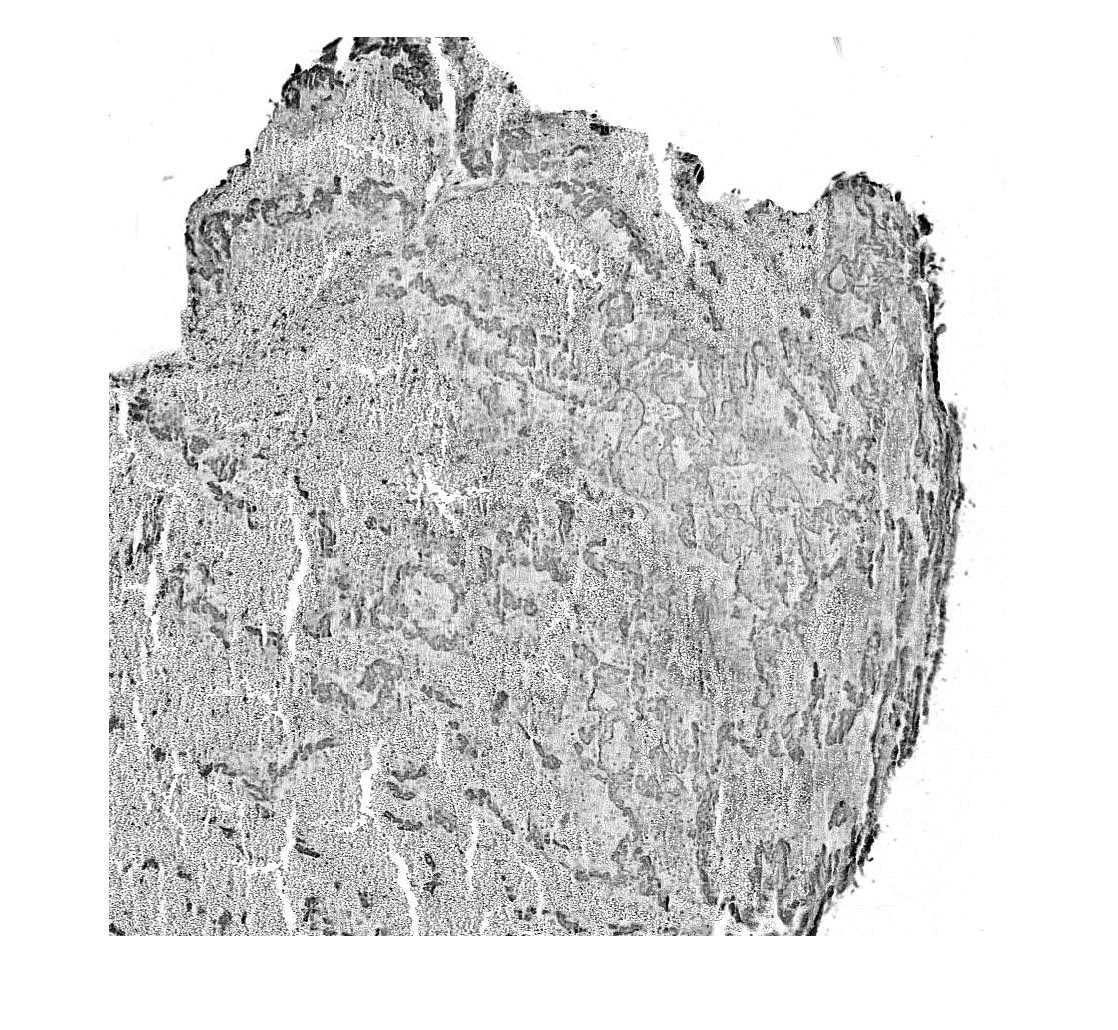
\includegraphics[width=4.5cm]{RGB_r}}}
	\qquad
	\subfloat[]{{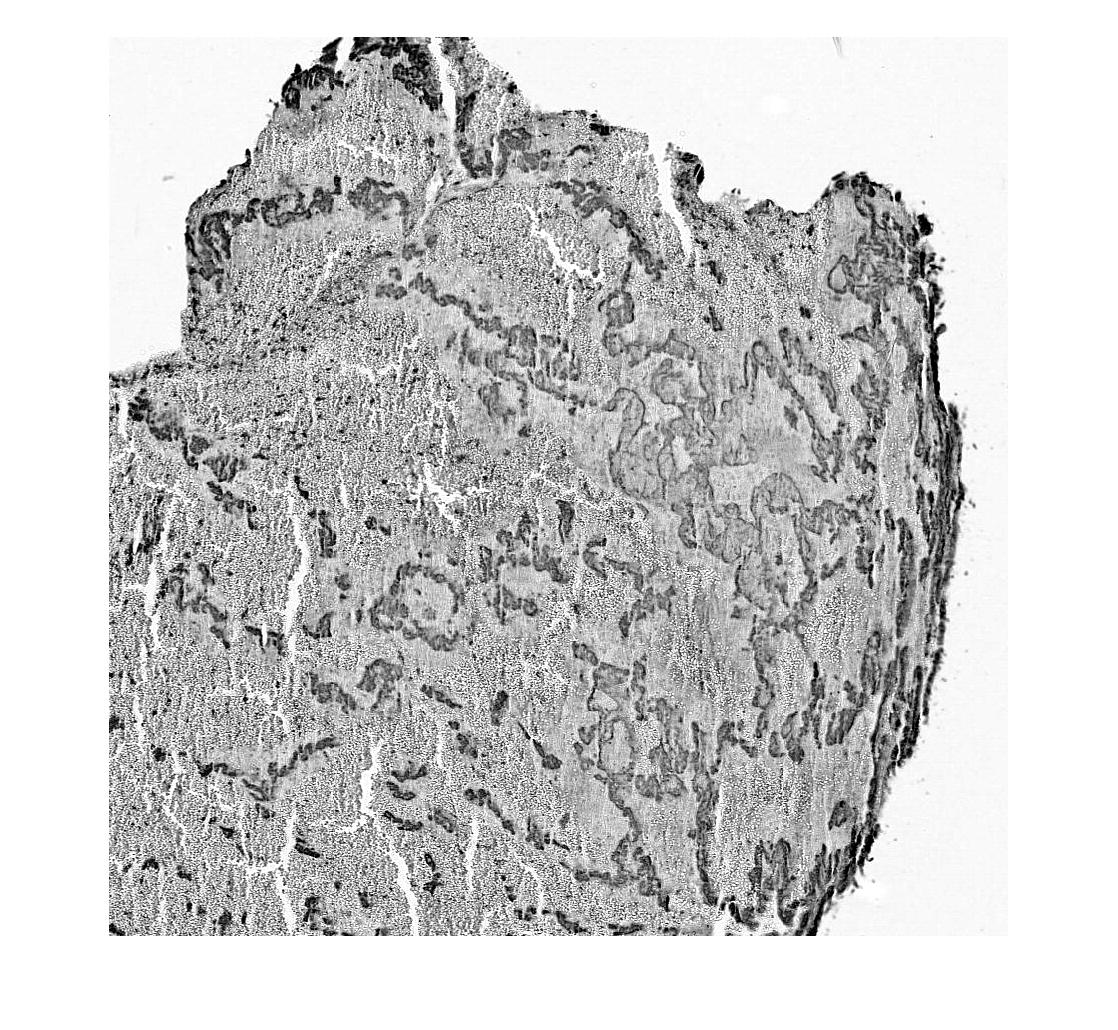
\includegraphics[width=4.5cm]{RGB_g}}}
	\qquad
	\subfloat[]{{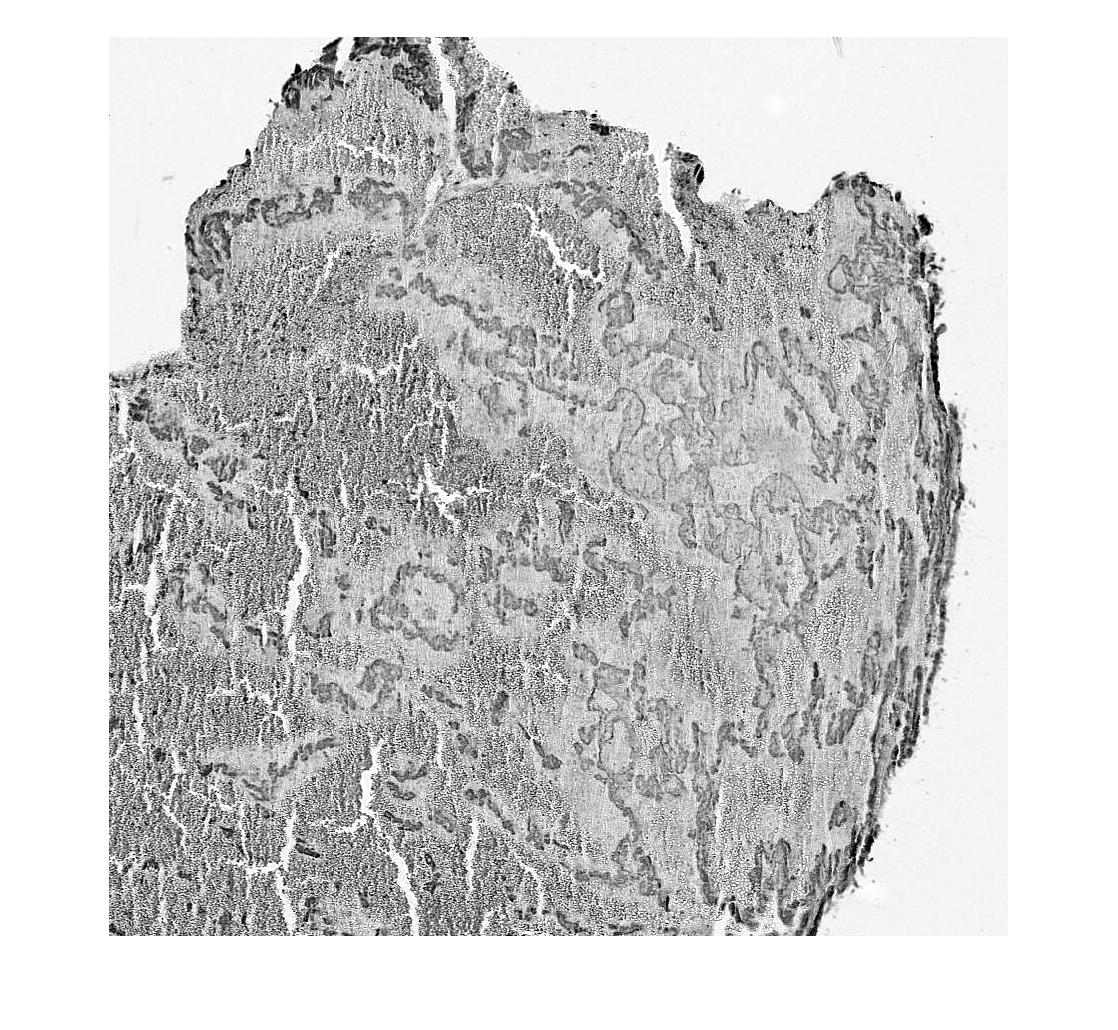
\includegraphics[width=4.5cm]{RGB_b}}}
	
	\caption{Illustratie van respectievelijk de rode, groene en blauwe kleurwaarden (RGB). Hierbij komt wit overeen met de maximumwaarde en zwart met de minimumwaarde van die kleur.}
	\label{figuur RGB}
\end{figure}

\begin{figure}[H]
	\centering
	\subfloat[]{{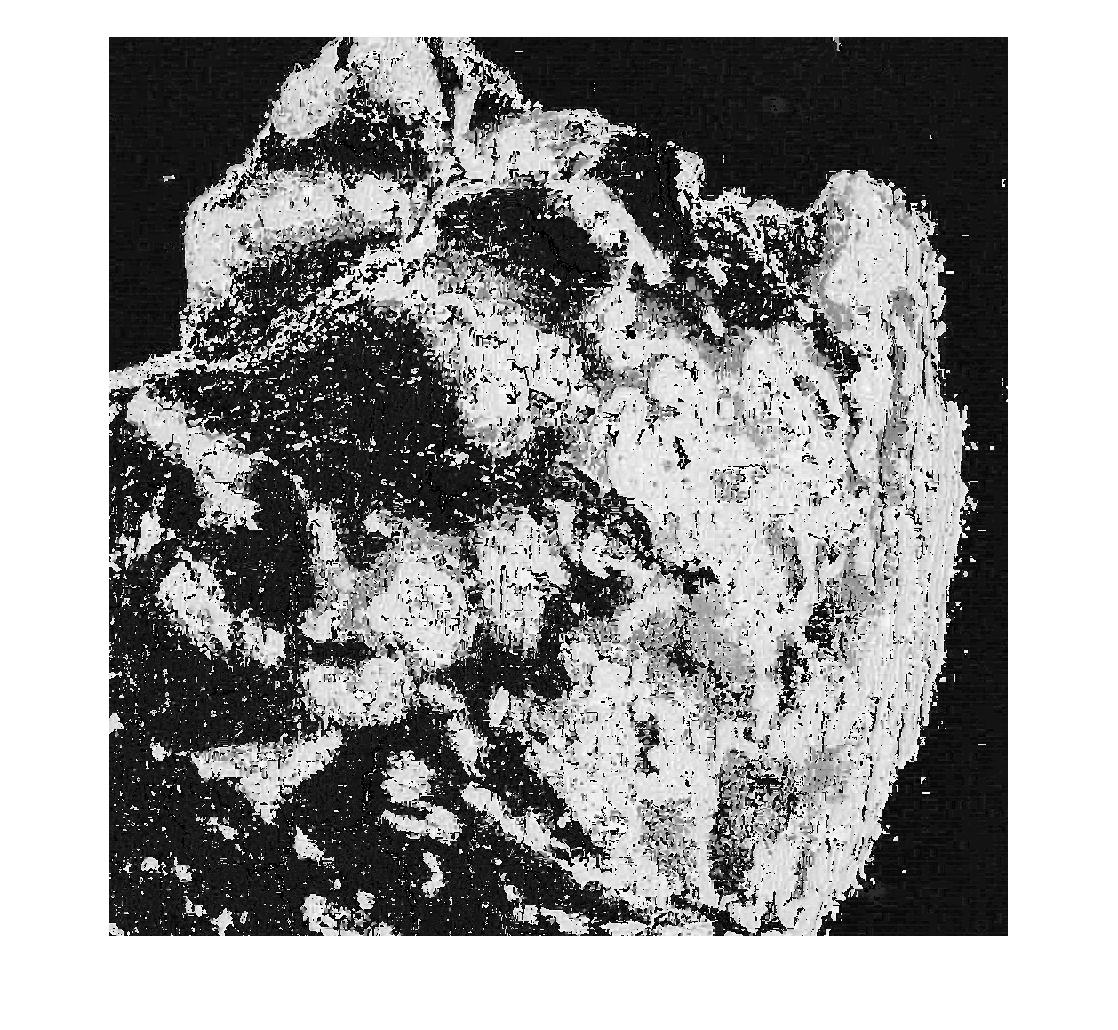
\includegraphics[width=4.5cm]{HSV_h}}}
	\qquad
	\subfloat[]{{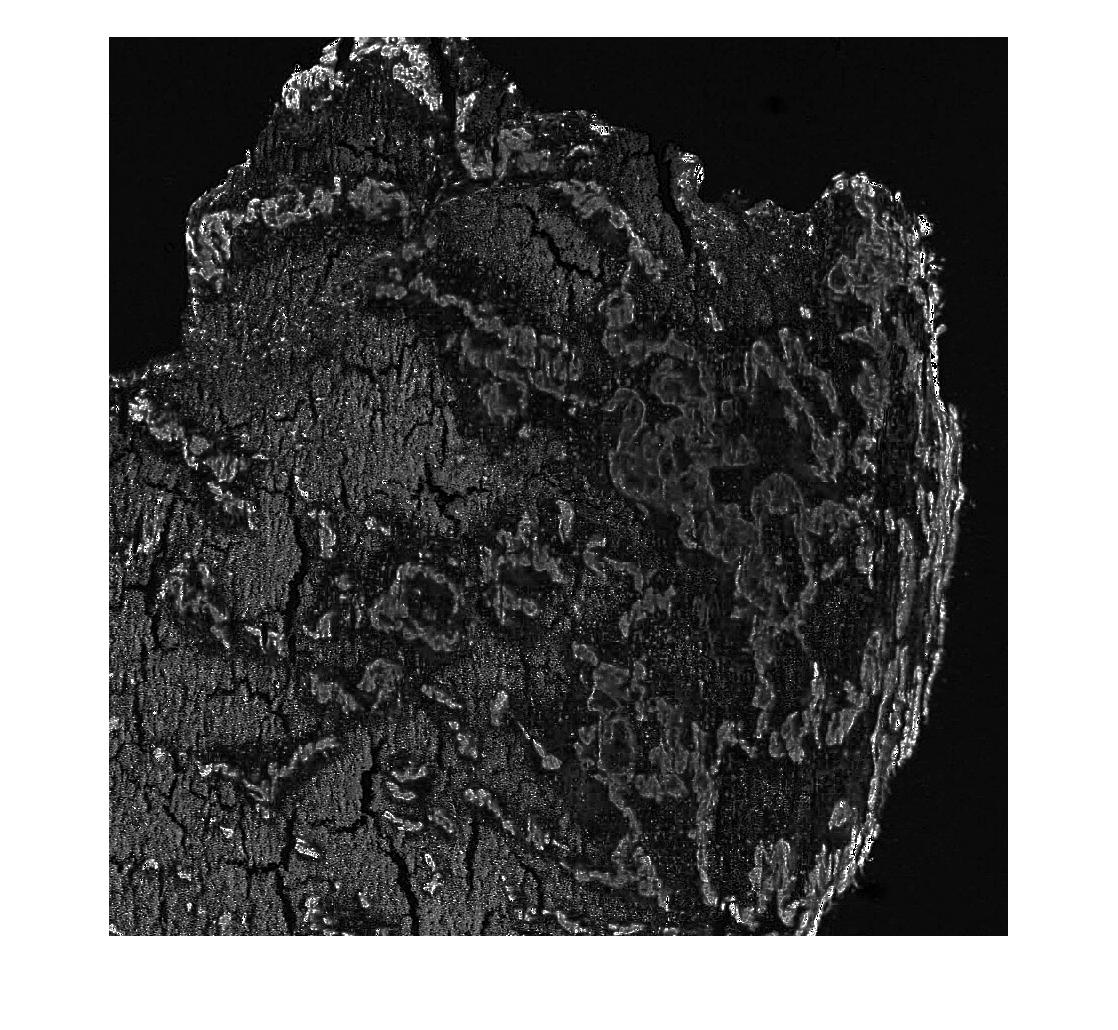
\includegraphics[width=4.5cm]{HSV_s}}}
	\qquad
	\subfloat[]{{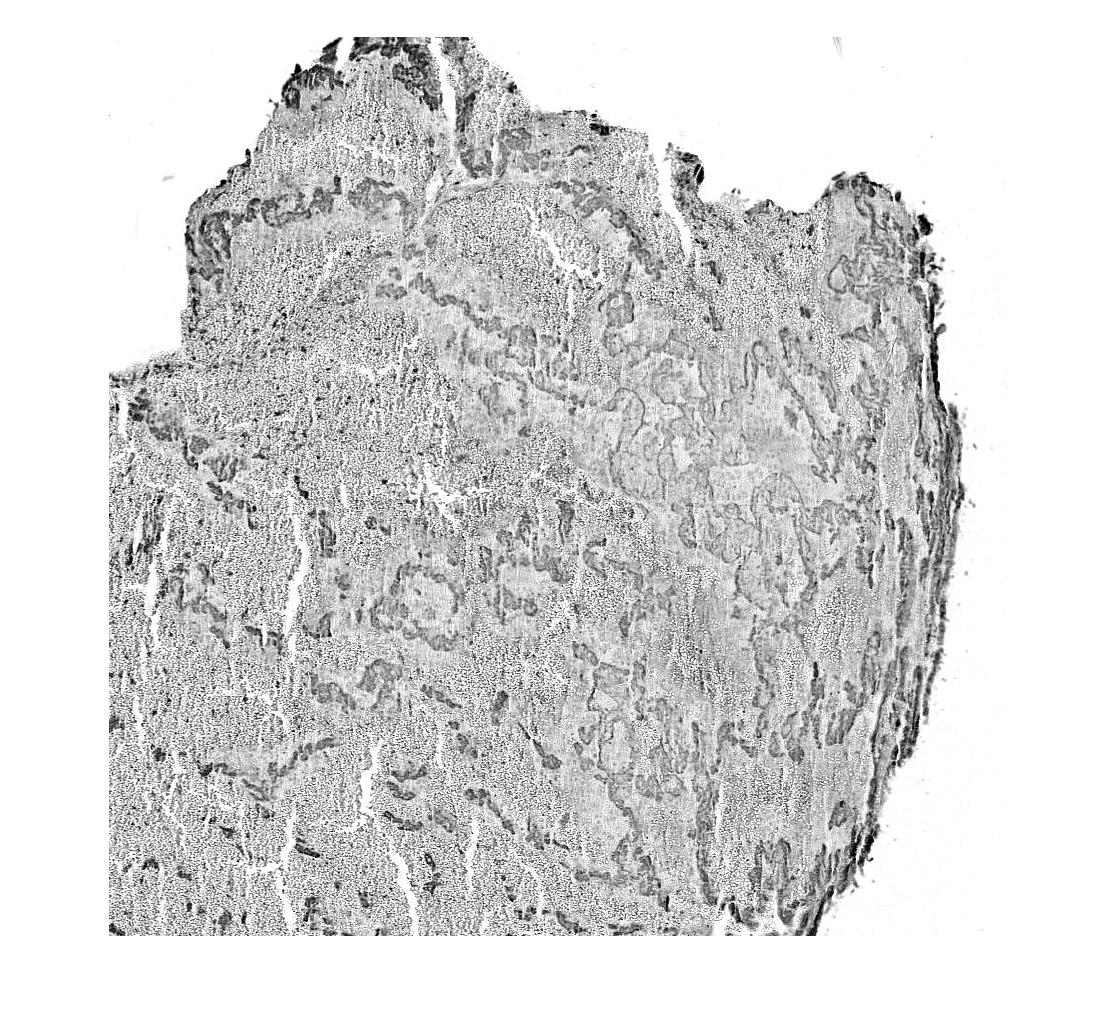
\includegraphics[width=4.5cm]{HSV_v}}}
	
	\caption{Illustratie van respectievelijk de hue, saturation en value kleurwaarden (HSV). Hierbij komt wit overeen met de maximumwaarde en zwart met de minimumwaarde van die kleurwaarde.}
	\label{figuur HSV}
\end{figure}

\subsubsection{Een algemene treshold}
De volgende stap is nu een filter bepalen voor alle indicatorpixels. Het probleem is echter dat een goede filter voor de ene foto niet altijd een goede filter voor de andere foto is. Daarom hebben we voor iedere foto manueel een 'treshold' bepaald en deze achteraf met elkaar vergeleken. Het resultaat is een vrij algemene treshold die alle indicatorpixels met zekerheid aanduidt. Af en toe worden jammer genoeg verkeerde pixels aangeduid. Het aantal is weliswaar niet zo groot, maar zullen we trachten te omzeilen in het volgende hoofdstuk. Een voorbeeld van deze algemene treshold is te zien op de volgende figuur:

\begin{figure}[H]
	\centering
	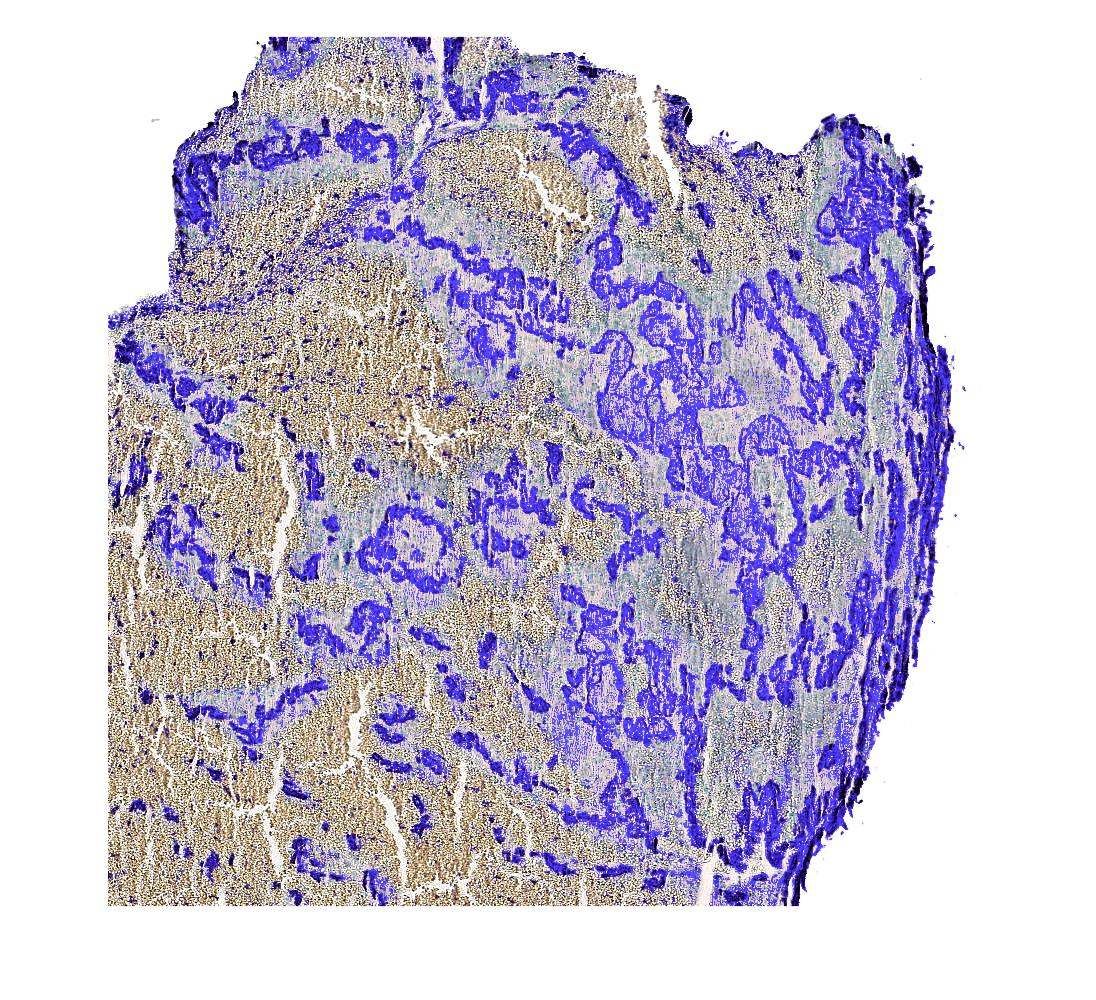
\includegraphics[width = 0.7\textwidth]{algemene_treshold}
	
	\caption{We hebben alle indicatoren met een blauwachtige kleur aangeduid. De algemene treshold selecteert alle indicatorpixels, maar jammer genoeg ook enkele verkeerde (voornamelijk rechtsonder).}
	\label{figuur alg_tresh}
\end{figure}

\subsubsection{Optimalisatie van de treshold}
In dit hoofdstuk willen we het aantal verkeerde pixels verminderen zonder de juiste te beïnvloeden. We hebben echter al een vrij goede treshold waardoor we een statistische analyse van wat onder deze mask ligt, kunnen uitvoeren. We stellen hiervoor een frequentiediagram van de \textit{HSV} kleurwaarden onder de mask op. Het levert ons namelijk een interessant resultaat dat te zien is in figuur  \ref{figuur HSVHIST}. We zien namelijk duidelijke verschillen in de frequenties van de kleurwaarden. \\
Het idee is om nu de verkeerde pixels via deze diagrammen eruit te filteren. Indien we veronderstellen dat de frequenties van deze specifieke pixels laag zijn en dat de verkeerde pixels in kleur verschillen met de indicatorpixels. Dan kunnen we in principe alle pixels met een frequentie onder een bepaalde grenswaarde schrappen. Een betere benadering is misschien om het punt te vinden, waar de frequentie van de pixels enorm begint toe te nemen of we met andere woorden grote 'indicatoraders' aan het verwijderen zijn. Dit punt kan theoretisch benaderd worden als het maximum van de tweede afgeleide naar de kleurwaarde. Jammer genoeg hebben we de tijd nog niet gehad om dit idee te testen. \\
Een mogelijk extra stap is om de indicatorpixels morfologisch te sluiten met een algoritme dat reeds in MATLAB verwerkt is. Indien we met onze filtering enkele holtes maken, kunnen deze dan zonder problemen worden opgevuld. Ter illustratie geven we het standaardvoorbeeld van MATLAB in figuur \ref{figuur morf} weer.


\begin{figure}[H]
	\centering
	\subfloat[]{{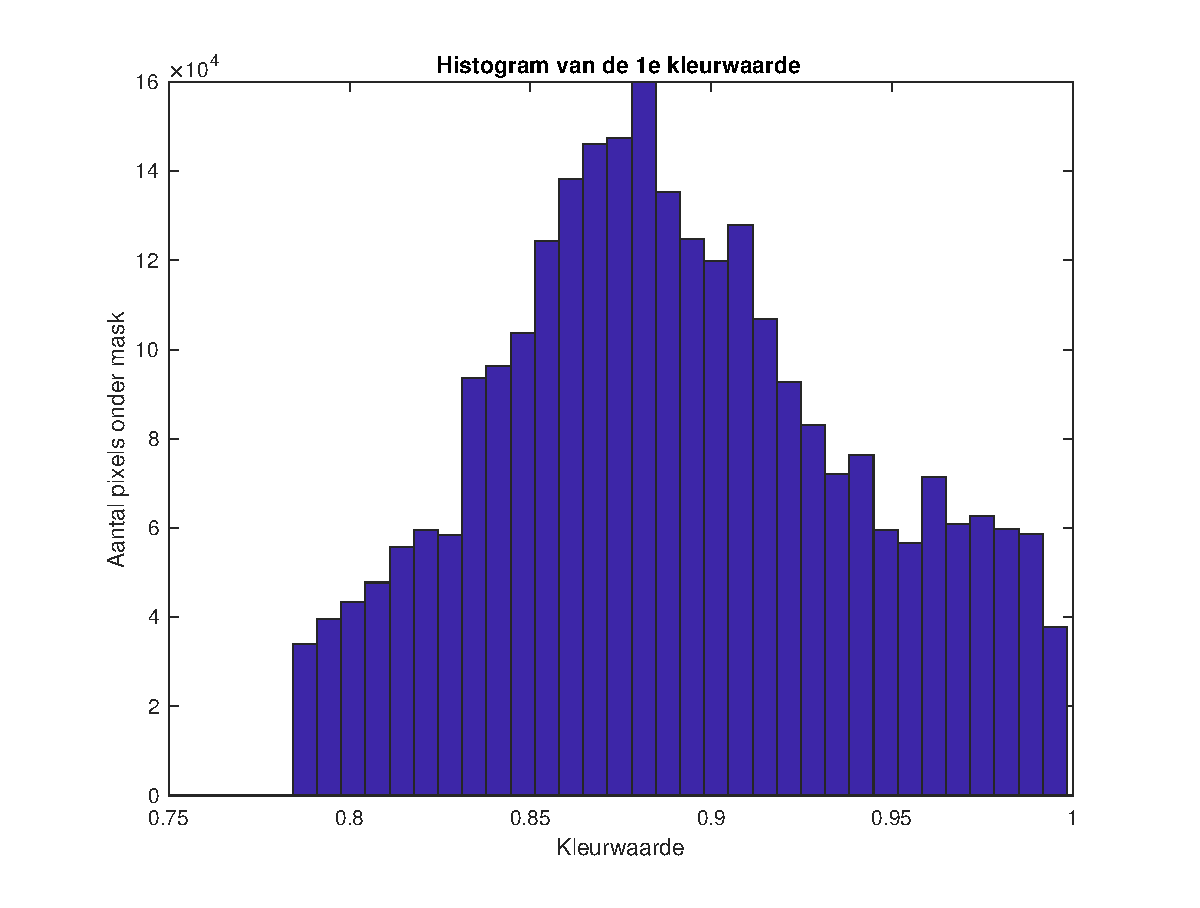
\includegraphics[width=4.5cm]{hsvhist_h}}}
	\qquad
	\subfloat[]{{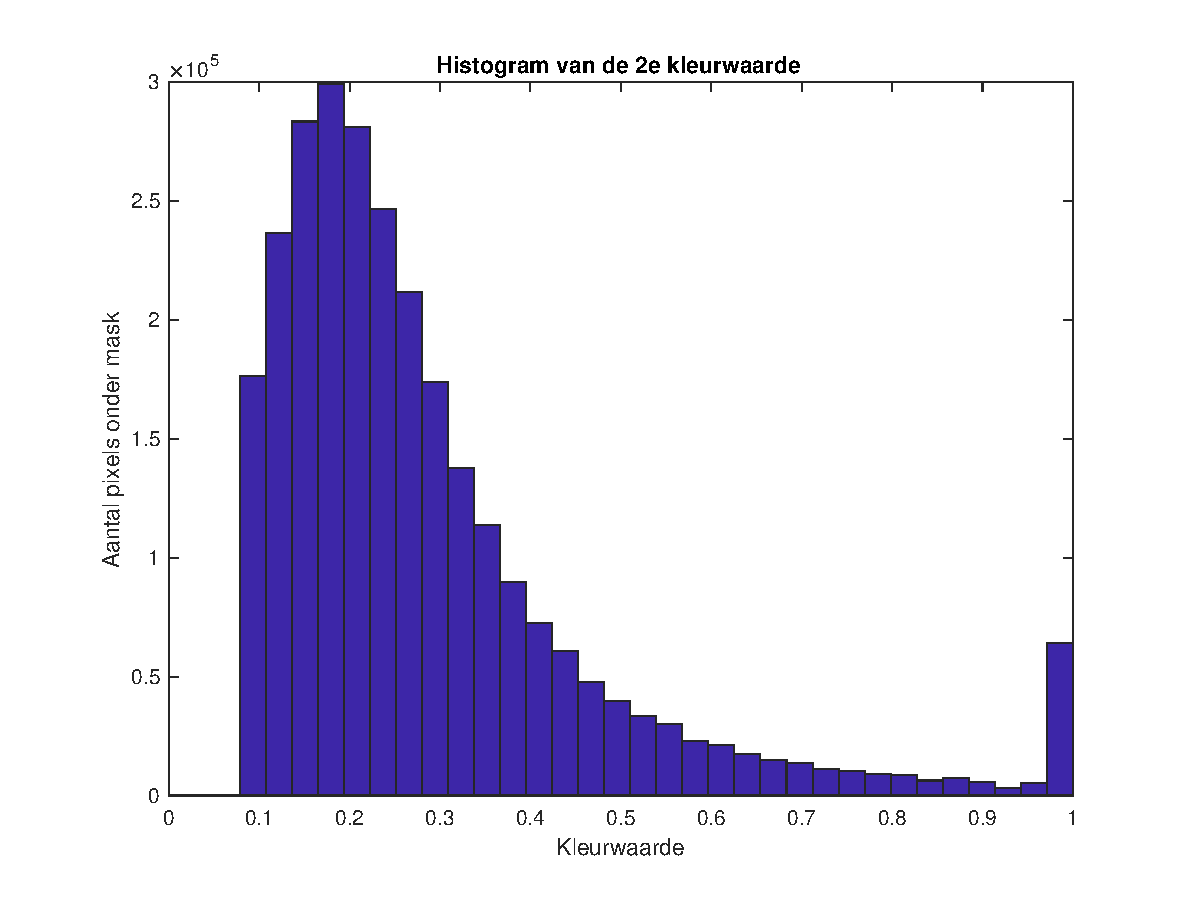
\includegraphics[width=4.5cm]{hsvhist_s}}}
	\qquad
	\subfloat[]{{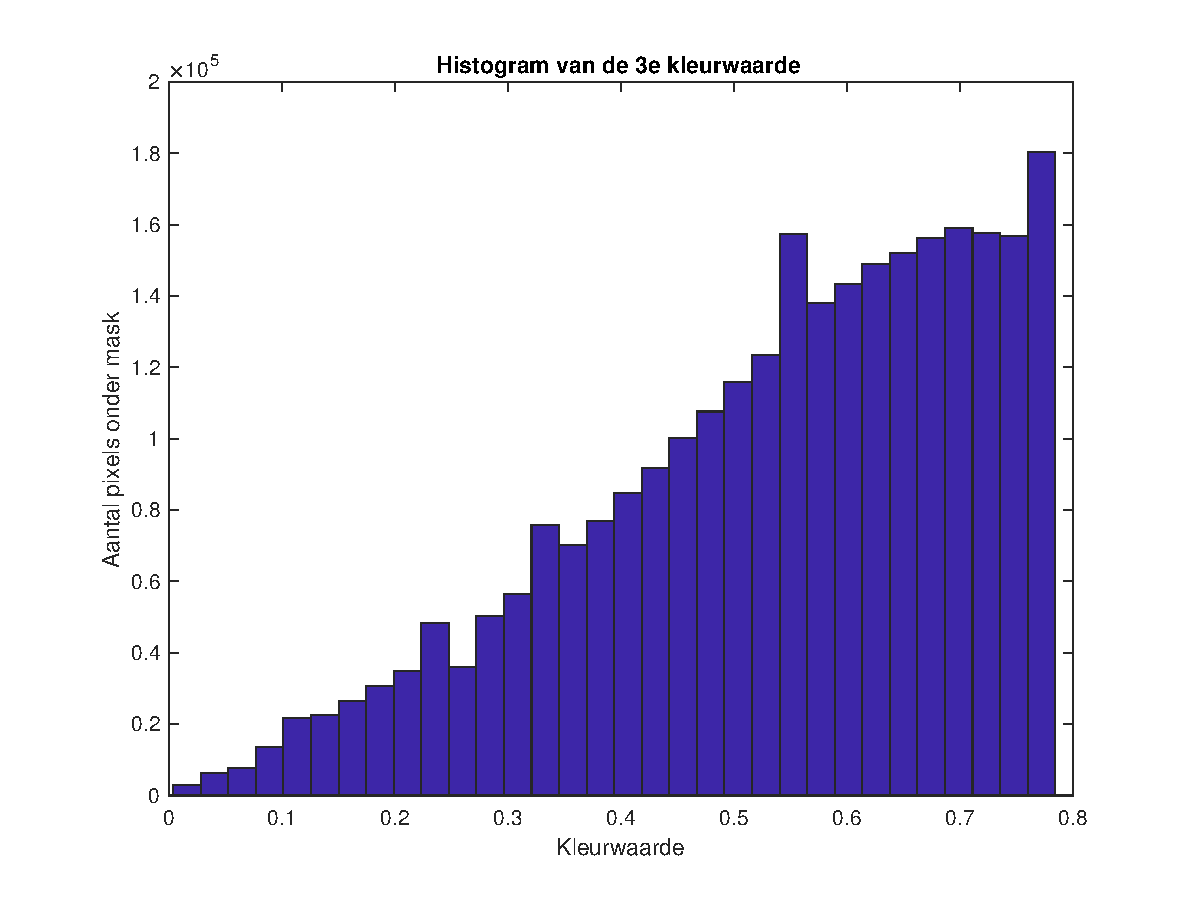
\includegraphics[width=4.5cm]{hsvhist_v}}}
	
	\caption{Histogrammen van de HSV kleurwaarden. We zien duidelijk het verschil in frequenties}
	\label{figuur HSVHIST}
\end{figure}

\begin{figure}[H]
	\centering
	\subfloat[]{{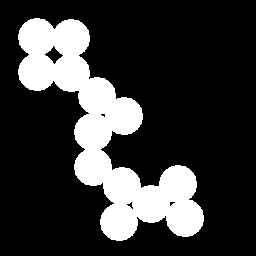
\includegraphics[width=7.5cm]{morf_open}}}
	\qquad
	\subfloat[]{{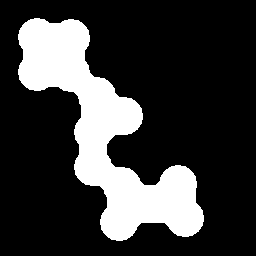
\includegraphics[width=7.5cm]{morf_gesloten}}}
	
	\caption{Illustratie waarbij de witte cirkels uit afbeelding (a) morfologisch gesloten worden in afbeelding (b)}
	\label{figuur morf}
\end{figure}

\subsection{De gebruiksvriendelijke applicatie}

\section*{Besluit}

Afsluitende tekst

\end{document}
